\documentclass[a4paper, 12pt]{article}


\usepackage{/Users/zhengz/Desktop/Math/Workspace/Homework1/homework}
%%%%%%%%%%%%%%%%%%%%%%%%%%%%%%%%%%%%%%%%%%%%%%%%%%%%%%%%%%%%%%%%%%%%%%%%%%%%%%%%%%%%%%%%%%%%%%%%%%%%%%%%%%%%%%%%%%%%%%%%%%%%%%%%%%%%%%%%
\begin{document}
%Header-Make sure you update this information!!!!
\noindent
%%%%%%%%%%%%%%%%%%%%%%%%%%%%%%%%%%%%%%%%%%%%%%%%%%%%%%%%%%%%%%%%%%%%%%%%%%%%%%%%%%%%%%%%%%%%%%%%%%%%%%%%%%%%%%%%%%%%%%%%%%%%%%%%%%%%%%%%
\large\textbf{Zhengdong Zhang} \hfill \textbf{Homework 9}   \\
Email: zhengz@uoregon.edu \hfill ID: 952091294 \\
\normalsize Course: MATH 635 - Algebraic Topology II \hfill Term: Winter 2025\\
Instructor: Dr.Daniel Dugger \hfill Due Date: $13^{th}$ March, 2025 \\
\noindent\rule{7in}{2.8pt}
\setstretch{1.1}

%%%%%%%%%%%%%%%%%%%%%%%%%%%%%%%%%%%%%%%%%%%%%%%%%%%%%%%%%%%%%%%%%%%%%%%%%%%%%%%%%%%%%%%%%%%%%%%%%%%%%%%%%%%%%%%%%%%%%%%%%%%%%%%%%%%%%%%%
%Probelm 1 
%%%%%%%%%%%%%%%%%%%%%%%%%%%%%%%%%%%%%%%%%%%%%%%%%%%%%%%%%%%%%%%%%%%%%%%%%%%%%%%%%%%%%%%%%%%%%%%%%%%%%%%%%%%%%%%%%%%%%%%%%%%%%%%%%%%%%%%%
\begin{problem}{1}
\begin{enumerate}[(a)]
\item Let \(p_1:S^1\rightarrow S^1\) and \(p_2:S^1\rightarrow S^1\) be given by \(p_1(z)=z^{15}\) and \(p_2(z)=z^6\). Is there a continous map \(f:S^1\rightarrow S^1\) making the diagram 
% https://q.uiver.app/#q=WzAsMyxbMCwwLCJTXjEiXSxbMiwwLCJTXjEiXSxbMSwxLCJTXjEiXSxbMCwyLCJwXzEiLDJdLFsxLDIsInBfMiJdLFswLDEsImYiXV0=
\[\begin{tikzcd}
	{S^1} && {S^1} \\
	& {S^1}
	\arrow["f", from=1-1, to=1-3]
	\arrow["{p_1}"', from=1-1, to=2-2]
	\arrow["{p_2}", from=1-3, to=2-2]
\end{tikzcd}\]
commute? Explain why or why not.
\item If \(T\) is the torus, use covering space theory to prove that every map \(\mathbb{R}P^5\rightarrow T\) is homotopic to a constant map.
\end{enumerate}
\end{problem}
\begin{solution}
\begin{enumerate}[(a)]
\item This is impossible. We know that \(\deg p_1=15\) and \(\deg p_2=6\). If such a map \(f:S^1\rightarrow S^1\) exists, then we have \(p_2\circ f=p_1\). This implies that 
\[(\deg p_2)(\deg f)=\deg p_1.\]
Thus, \(\deg f=15/6\notin \mathbb{Z}\). This contradicts the definition of degree.
\item Given a map \(f:\mathbb{R}P^5\rightarrow T\), note that \(\mathbb{R}P^5\) and \(T\) are path-connected, so we can viewed \(f\) as a pointed map. \(\mathbb{R}P^5\) is pointed at \(x\), \(T\) is pointed at \(b\), and we have 
\(f(x)=b\). Let \(p:(\mathbb{R}^2,e)\rightarrow (T,b)\) be the universal covering space where \(e\in p^{-1}(b)\) is a point in the fiber over \(b\). The map \(f\) induces a map between fundamental groups 
\[f_*:\pi_1(\mathbb{R}P^5,x)\rightarrow \pi_1(T,b)\]
where \(\pi_1(\mathbb{R}P^5,x)\cong \mathbb{Z}/2 \mathbb{Z}\) and \(\pi_1(T,b)\cong \mathbb{Z}\). We know the group \(\mathbb{Z}\) has no torsion, so \(f_*\) must be the zero map. This implies 
\[f_*(\pi_1(\mathbb{R}P^5,x))=0\subseteq 0=p_*(\pi_1(\mathbb{R}^2, e))\]
since \(\mathbb{R}^2\) is simply connected. By the map lifting lemma, there exists a lifting \(\ti{f}:\mathbb{R}P^5\rightarrow \mathbb{R}^2\) such that \(p\circ \ti{f}=f\), namely the following diagram commutes: 
% https://q.uiver.app/#q=WzAsMyxbMCwxLCJcXG1hdGhiYntSfVBeNSJdLFsxLDEsIlQiXSxbMSwwLCJcXG1hdGhiYntSfV4yIl0sWzIsMSwicCJdLFswLDEsImYiLDJdLFswLDIsIlxcdGlsZGV7Zn0iLDAseyJzdHlsZSI6eyJib2R5Ijp7Im5hbWUiOiJkYXNoZWQifX19XV0=
\[\begin{tikzcd}
	& {\mathbb{R}^2} \\
	{\mathbb{R}P^5} & T
	\arrow["p", from=1-2, to=2-2]
	\arrow["{\tilde{f}}", dashed, from=2-1, to=1-2]
	\arrow["f"', from=2-1, to=2-2]
\end{tikzcd}\]
We know that \(\mathbb{R}^2\) is contractible, by the convexity lemma, \(\ti{f}\) is nullhomotopic. There exists \(H:\mathbb{R}P^5\times I\rightarrow \mathbb{R}^2\) such that \(H(-,0)=\ti{f}\) and \(H(-,1)=C_e\) the constant map. The composition 
\(p\circ H:\mathbb{R}P^5\times I\rightarrow T\) gives a homotopy between \(f\) and the constant map \(C_b\). This proves that \(f\) is nullhomotopic.
\end{enumerate}
\end{solution}

\noindent\rule{7in}{2.8pt}
%%%%%%%%%%%%%%%%%%%%%%%%%%%%%%%%%%%%%%%%%%%%%%%%%%%%%%%%%%%%%%%%%%%%%%%%%%%%%%%%%%%%%%%%%%%%%%%%%%%%%%%%%%%%%%%%%%%%%%%%%%%%%%%%%%%%%%%%
%Probelm 2
%%%%%%%%%%%%%%%%%%%%%%%%%%%%%%%%%%%%%%%%%%%%%%%%%%%%%%%%%%%%%%%%%%%%%%%%%%%%%%%%%%%%%%%%%%%%%%%%%%%%%%%%%%%%%%%%%%%%%%%%%%%%%%%%%%%%%%%%
\begin{problem}{2}
Let \(B\) be the figure-eight space, with \(b\) the wedge point and basic loops \(\alpha\) and \(\beta\). We know that \(\pi_1(B,b)\) is the free group on the two generators 
\(\alpha\) and \(\beta\). Draw a picture showing the pointed covering space \(p:E\rightarrow B\) having \(p_*(\pi_1(E,e))=H\) for each of the following subgroups (in each case make clear what the basepoint \(e\) is in your picture).
\begin{enumerate}[(a)]
\item \(H=\la \alpha^2\ra\)
\item \(H=\la \alpha^2,\beta^2\ra\)
\item \(H=\la \alpha^2,\beta^2,(\alpha\beta)^3\ra\)
\item \(H=\la \alpha\beta,\alpha\beta^{-1}\ra \)
\end{enumerate}
\end{problem}
\begin{solution}
The pictures are as follows. The base point \(b\in B\) is the blue point, and the basepoint \(e\in E\) is the red point. All the preimage of \(b\) in \(E\) is the pink points. 
\[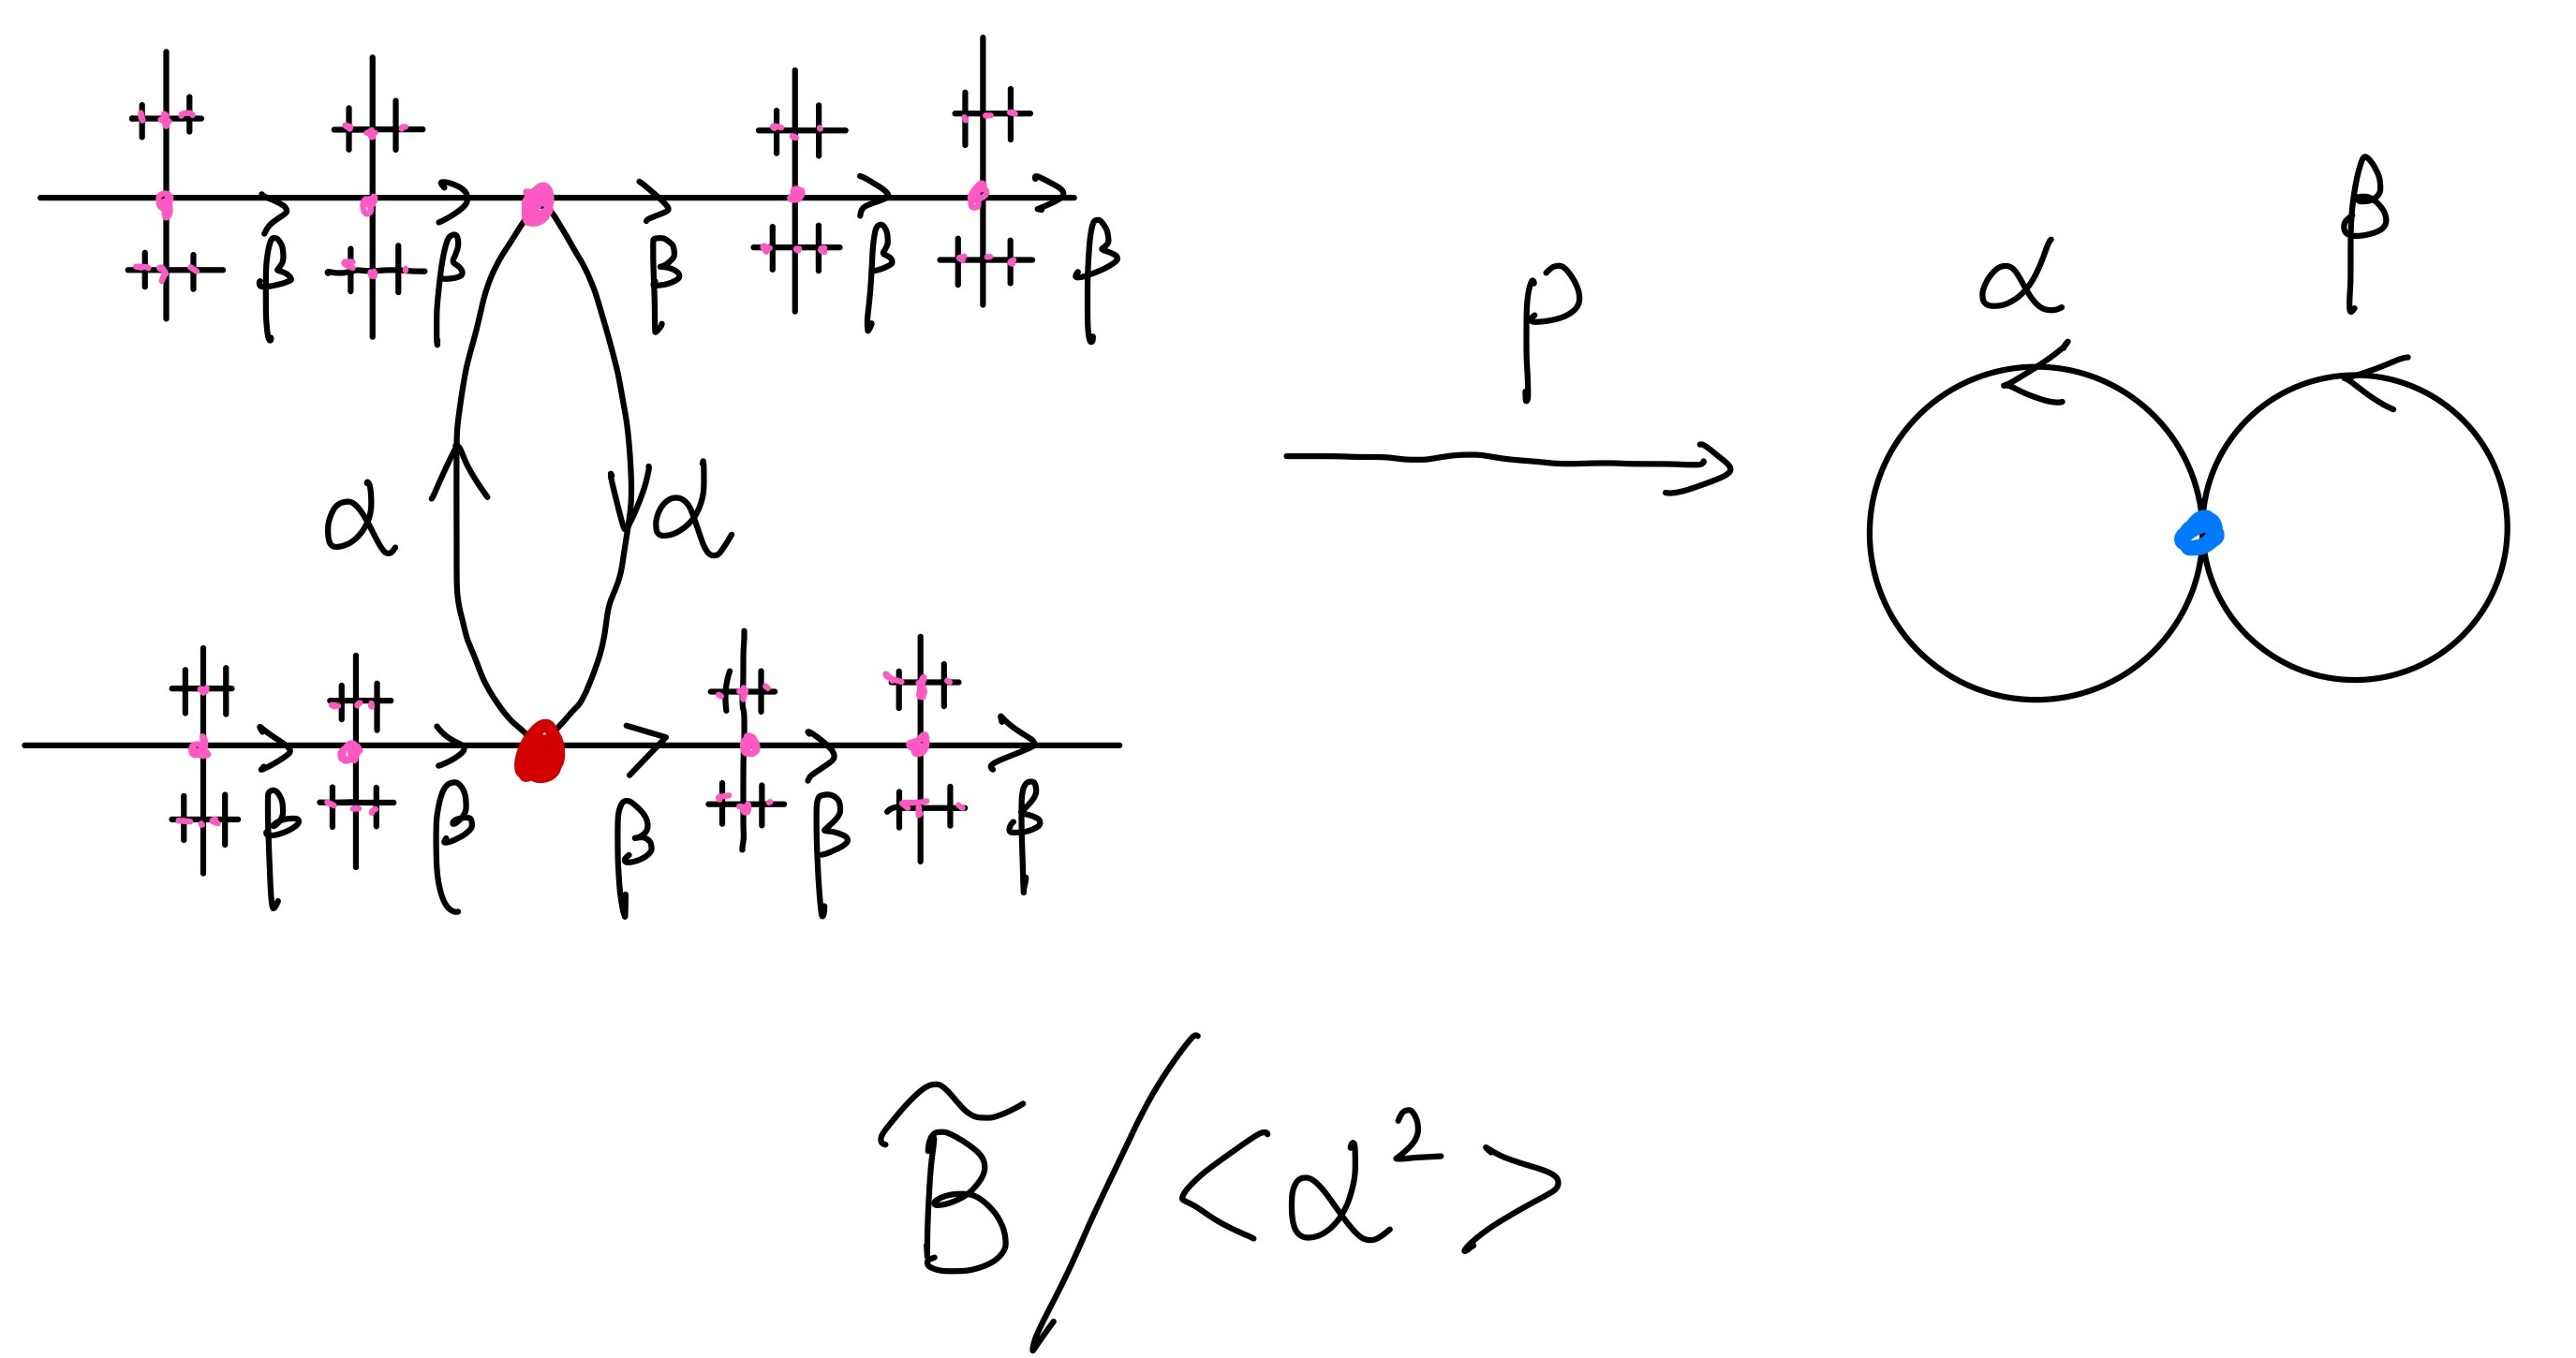
\includegraphics[scale=0.08]{Pictures/HW9-2-1.jpg}\]
\[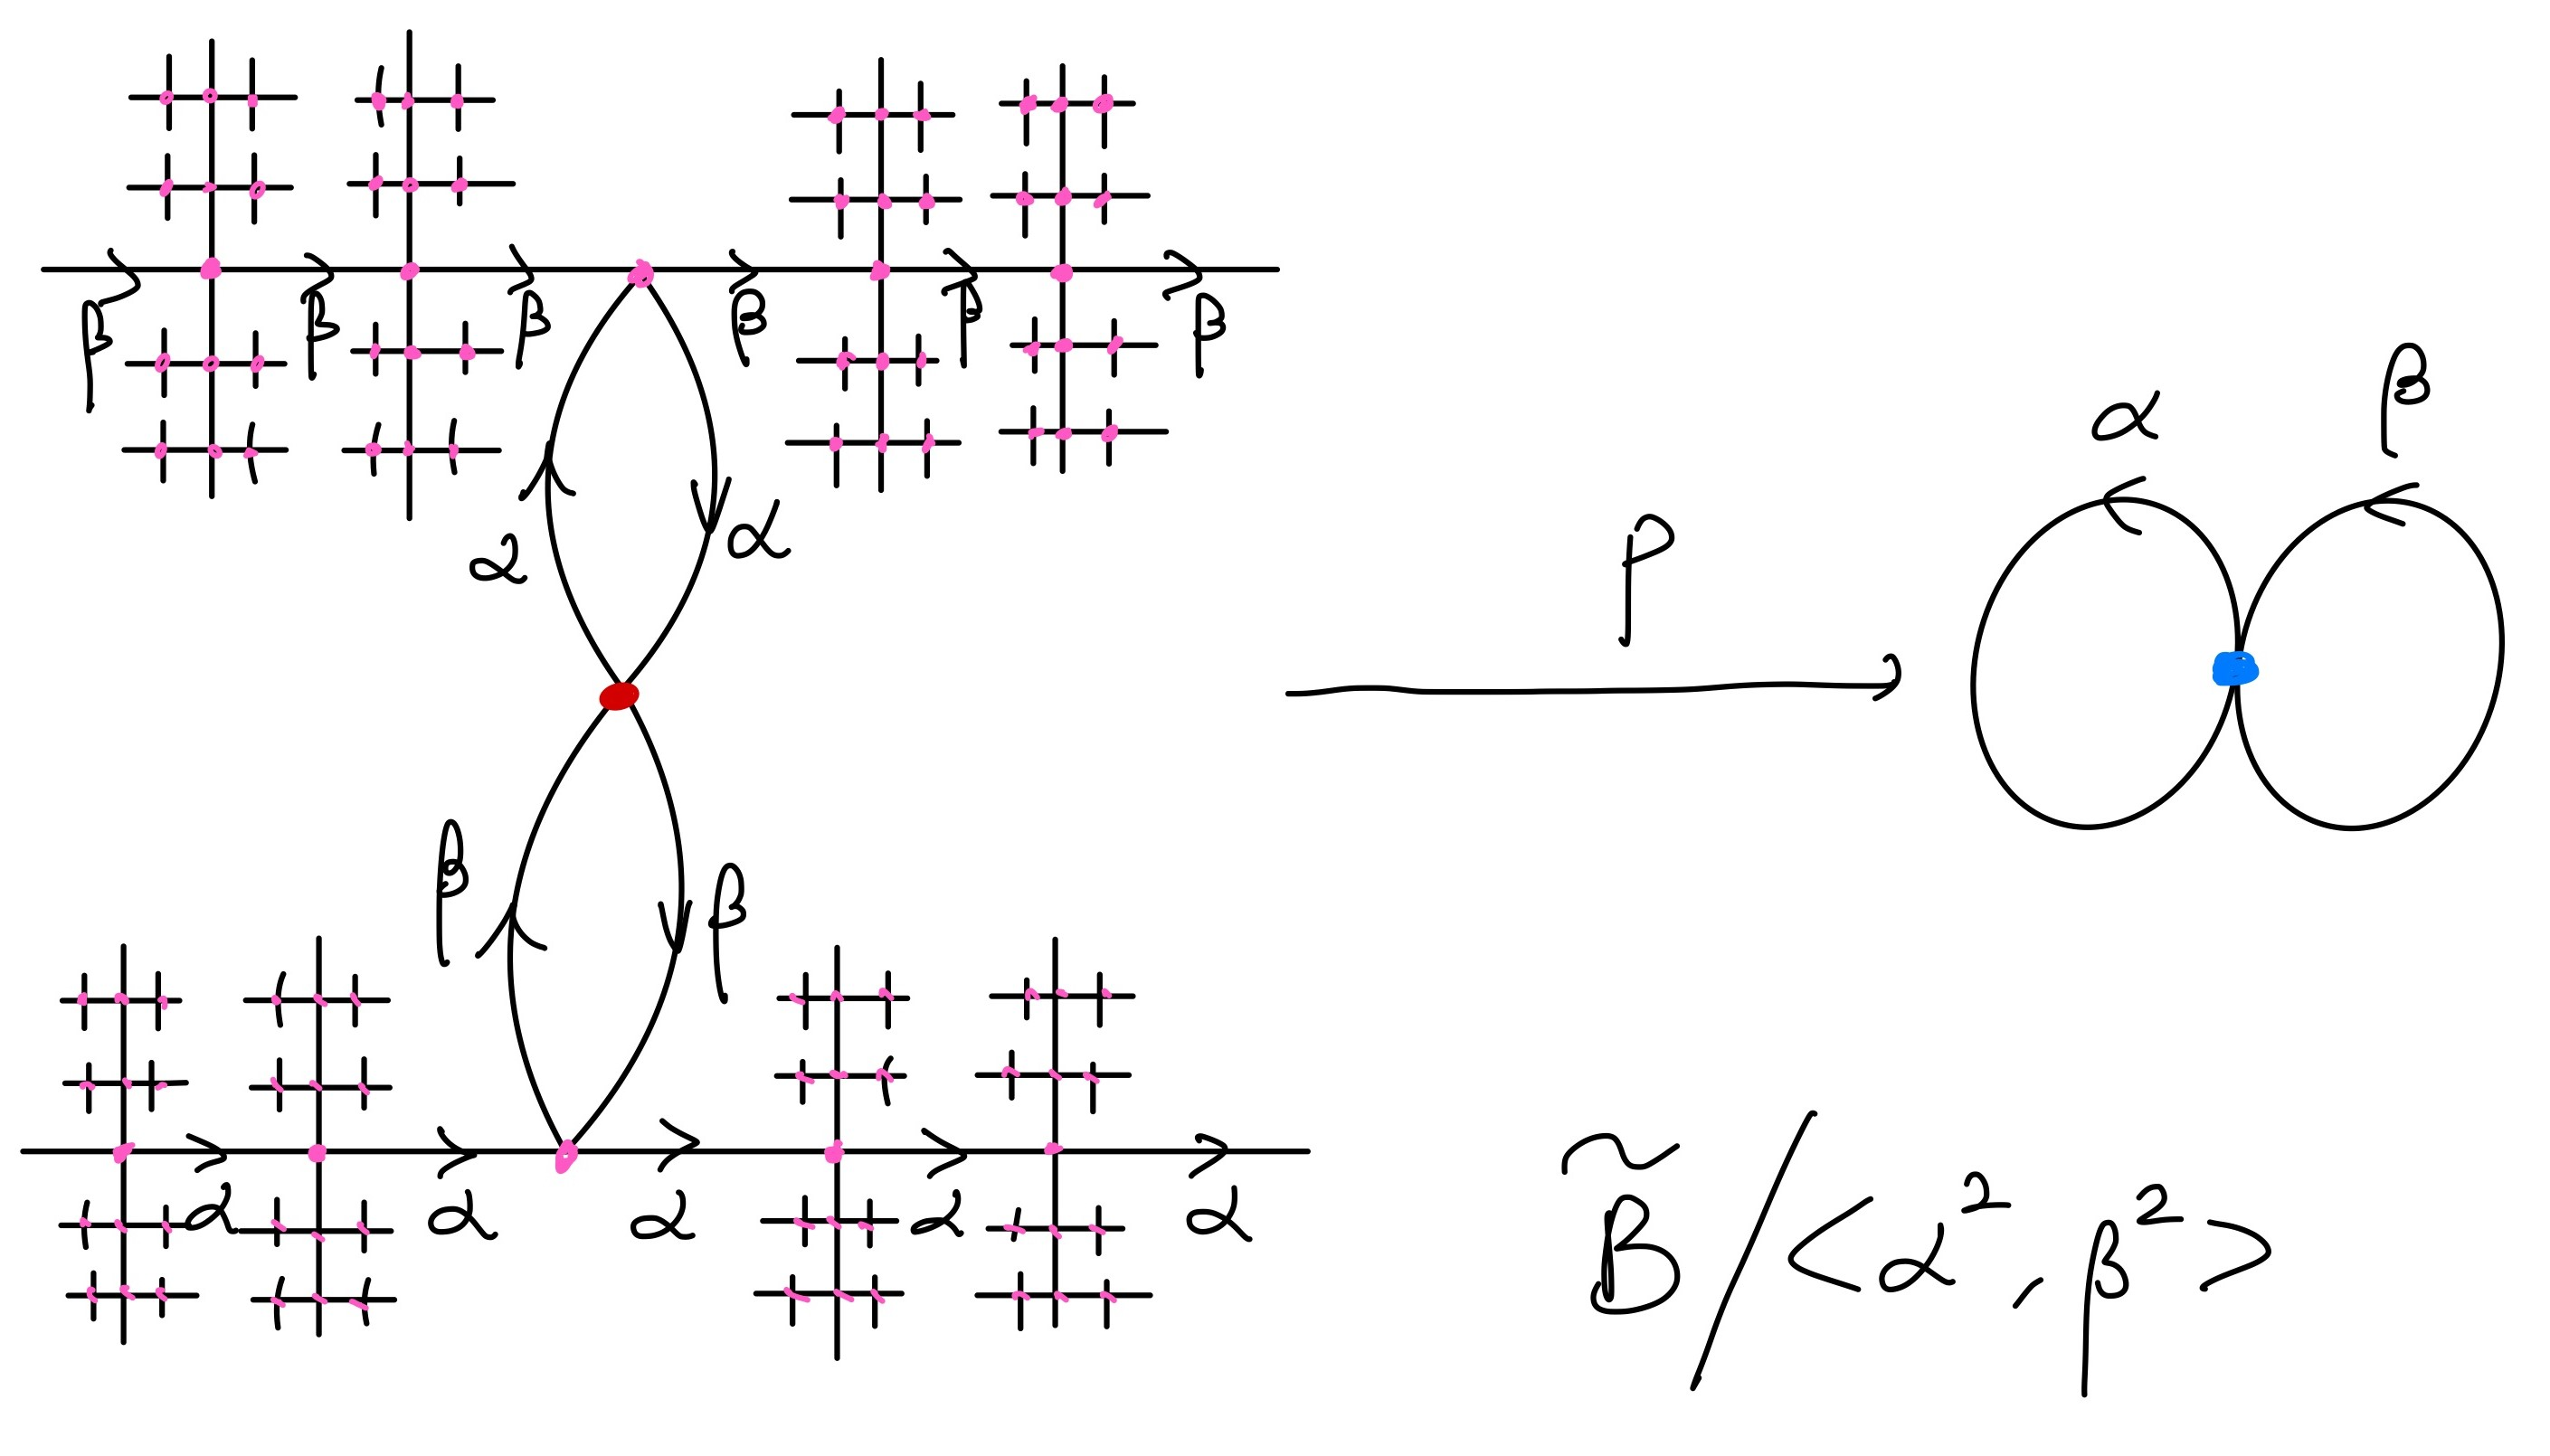
\includegraphics[scale=0.08]{Pictures/HW9-2-2.jpg}\]
\[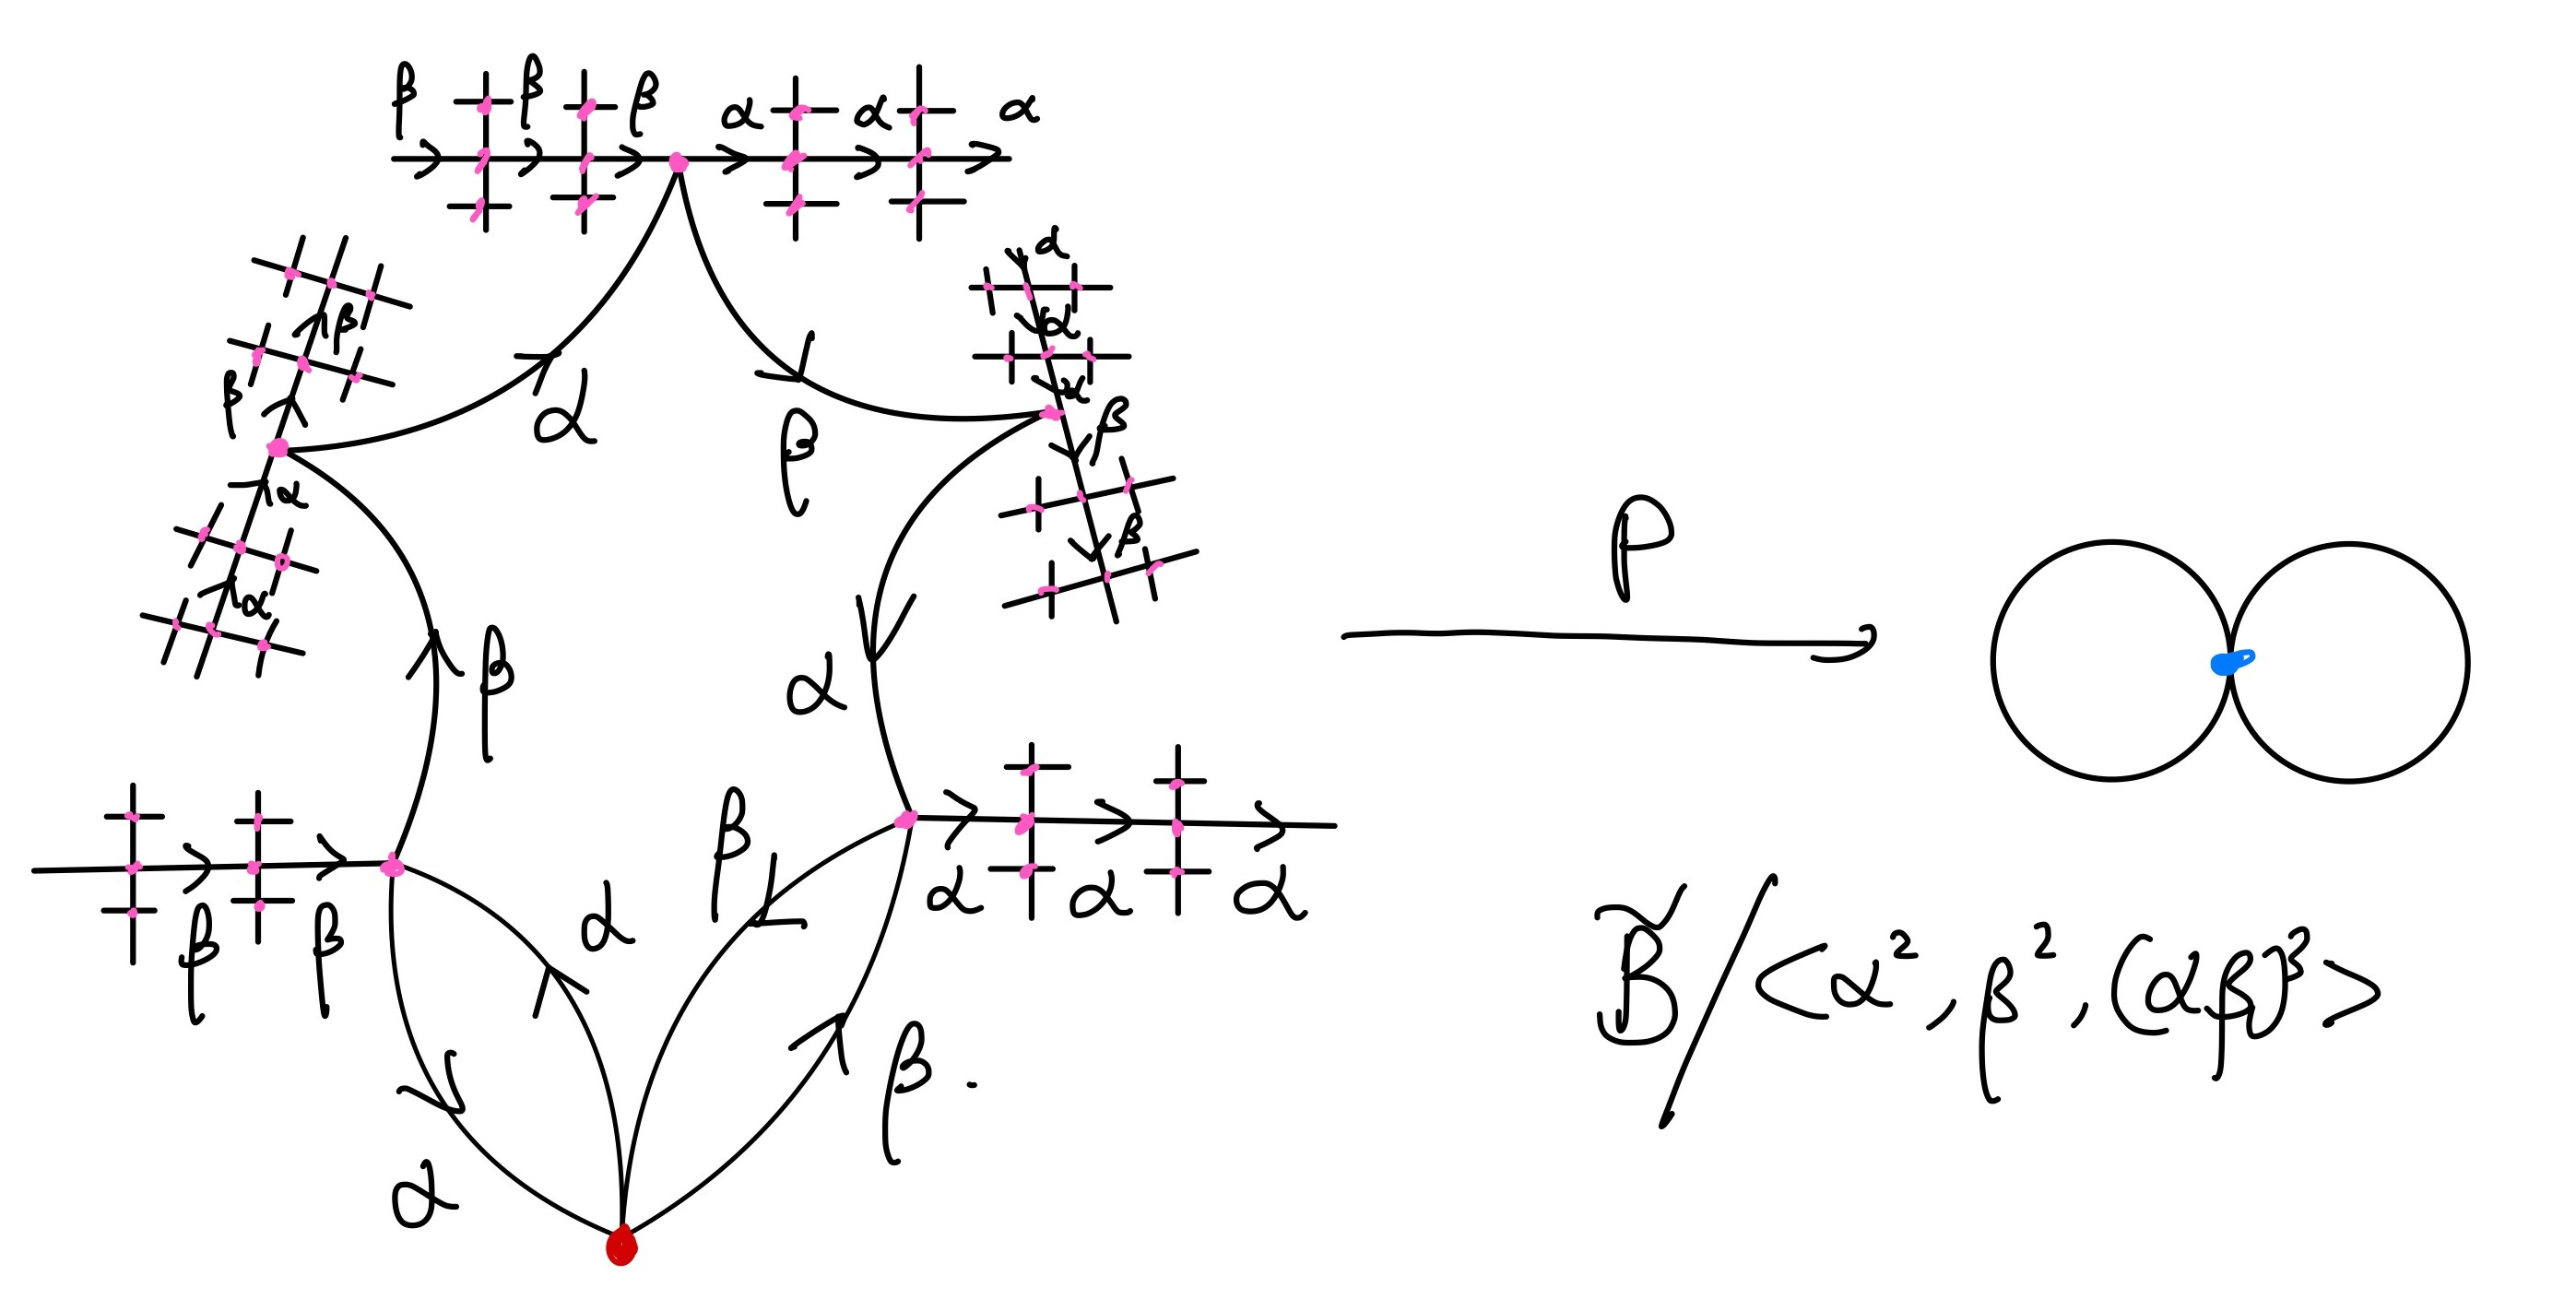
\includegraphics[scale=0.08]{Pictures/HW9-2-3.jpg}\]
\[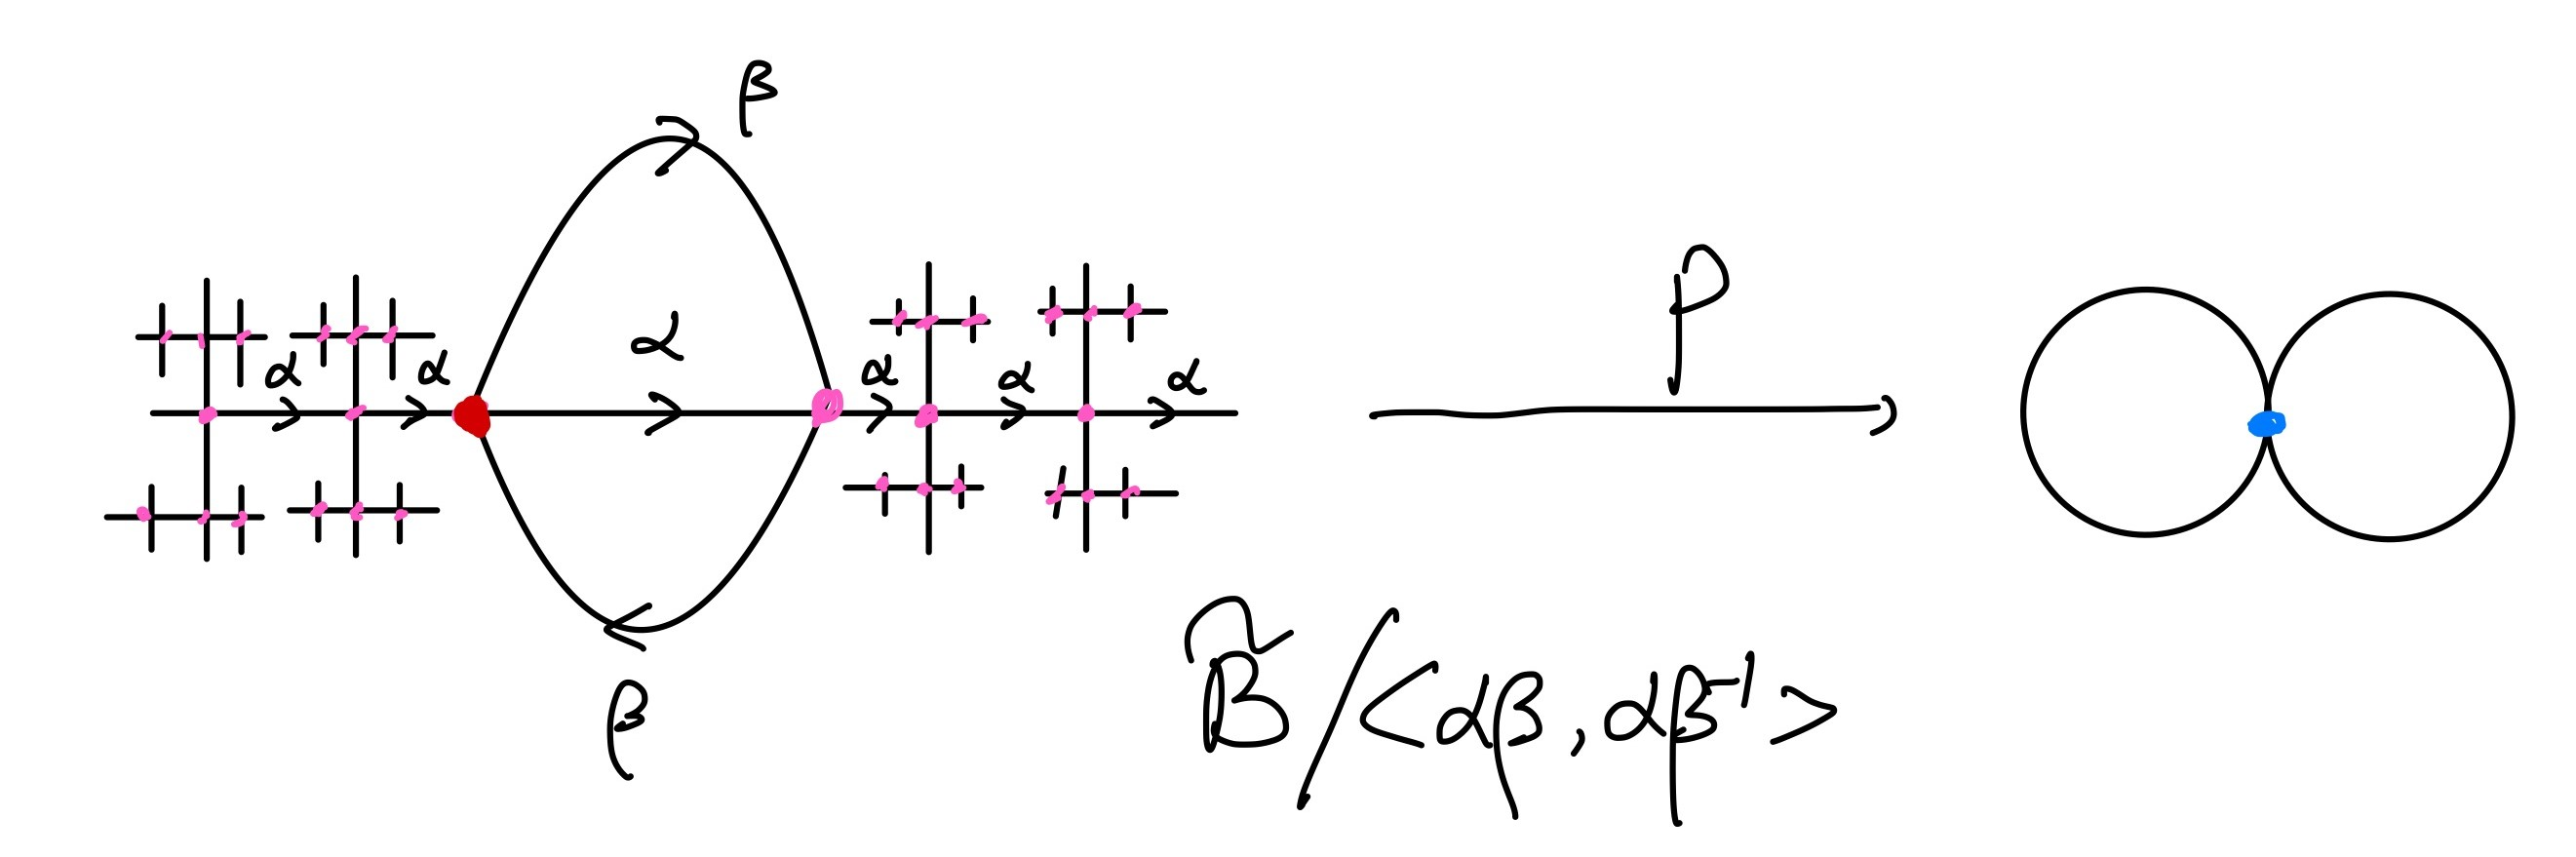
\includegraphics[scale=0.08]{Pictures/HW9-2-4.jpg}\]
\end{solution}

\noindent\rule{7in}{2.8pt}
%%%%%%%%%%%%%%%%%%%%%%%%%%%%%%%%%%%%%%%%%%%%%%%%%%%%%%%%%%%%%%%%%%%%%%%%%%%%%%%%%%%%%%%%%%%%%%%%%%%%%%%%%%%%%%%%%%%%%%%%%%%%%%%%%%%%%%%%
%Probelm 3 regular covering space
%%%%%%%%%%%%%%%%%%%%%%%%%%%%%%%%%%%%%%%%%%%%%%%%%%%%%%%%%%%%%%%%%%%%%%%%%%%%%%%%%%%%%%%%%%%%%%%%%%%%%%%%%%%%%%%%%%%%%%%%%%%%%%%%%%%%%%%%
\begin{problem}{3}
Recall the universal covering space for \(\mathbb{R}P^2\vee \mathbb{R}P^2\). 
\begin{enumerate}[(a)]
\item \(\mathbb{R}P^2\vee \mathbb{R}P^2\) has a regular \(8\)-fold covering space whose automorphism group is isomorphic to the dihedral group 
\[D_4=\la p,q\mid p^2=q^2=1,(pq)^4=1\ra.\]
Find the covering space and compute the homology groups. 
\item Given an example of a non-regular \(4\)-fold cover of \(\mathbb{R}P^2\vee \mathbb{R}P^2\).
\end{enumerate}
\end{problem}
\begin{solution}
\begin{enumerate}[(a)]
\item Let \(B=\mathbb{R}P^2\vee \mathbb{R}P^2\) and \(G=\pi_1(B)\cong \mathbb{Z}/2*\mathbb{Z}/2\) be the fundamental group. This is a regular covering, so we know that \(\Aut_B(E)=G/H\cong D_4\) for some normal subgroup \(H\unlhd G\). Let \(f:G\rightarrow D_4\) be the quotient map, we have a short exact sequence of groups 
% https://q.uiver.app/#q=WzAsNSxbMCwwLCIxIl0sWzEsMCwiSCJdLFsyLDAsIkciXSxbMywwLCJEXzQiXSxbNCwwLCIxIl0sWzAsMV0sWzEsMl0sWzIsMywiZiJdLFszLDRdXQ==
\[\begin{tikzcd}
	1 & H & G & {D_4} & 1
	\arrow[from=1-1, to=1-2]
	\arrow[from=1-2, to=1-3]
	\arrow["f", from=1-3, to=1-4]
	\arrow[from=1-4, to=1-5]
\end{tikzcd}\]
\(G\) is generated by 2 elements of order 2. Assume \(G\) and \(D_4\) have the following presentation
\begin{align*}
	G&=\la p,q\mid p^2=q^2=1\ra,\\ 
	D_4&=\la p,q\mid p^2=q^2=1,(pq)^4=1\ra.
\end{align*}
then \(f\) sends the generators \(p,q\) to \(p,q\). We can see that the kernel \(H=\la (pq)^4\ra\). So this regular 8-fold covering space is isomorphic to \(\ti{B}/\la (pq)^4\ra\) where \(\ti{B}\) is the universal covering space of \(B\). From 
the Homework\#8 we know that \(\ti{B}\) is an infinite wedge of \(2\)-spheres. 
\[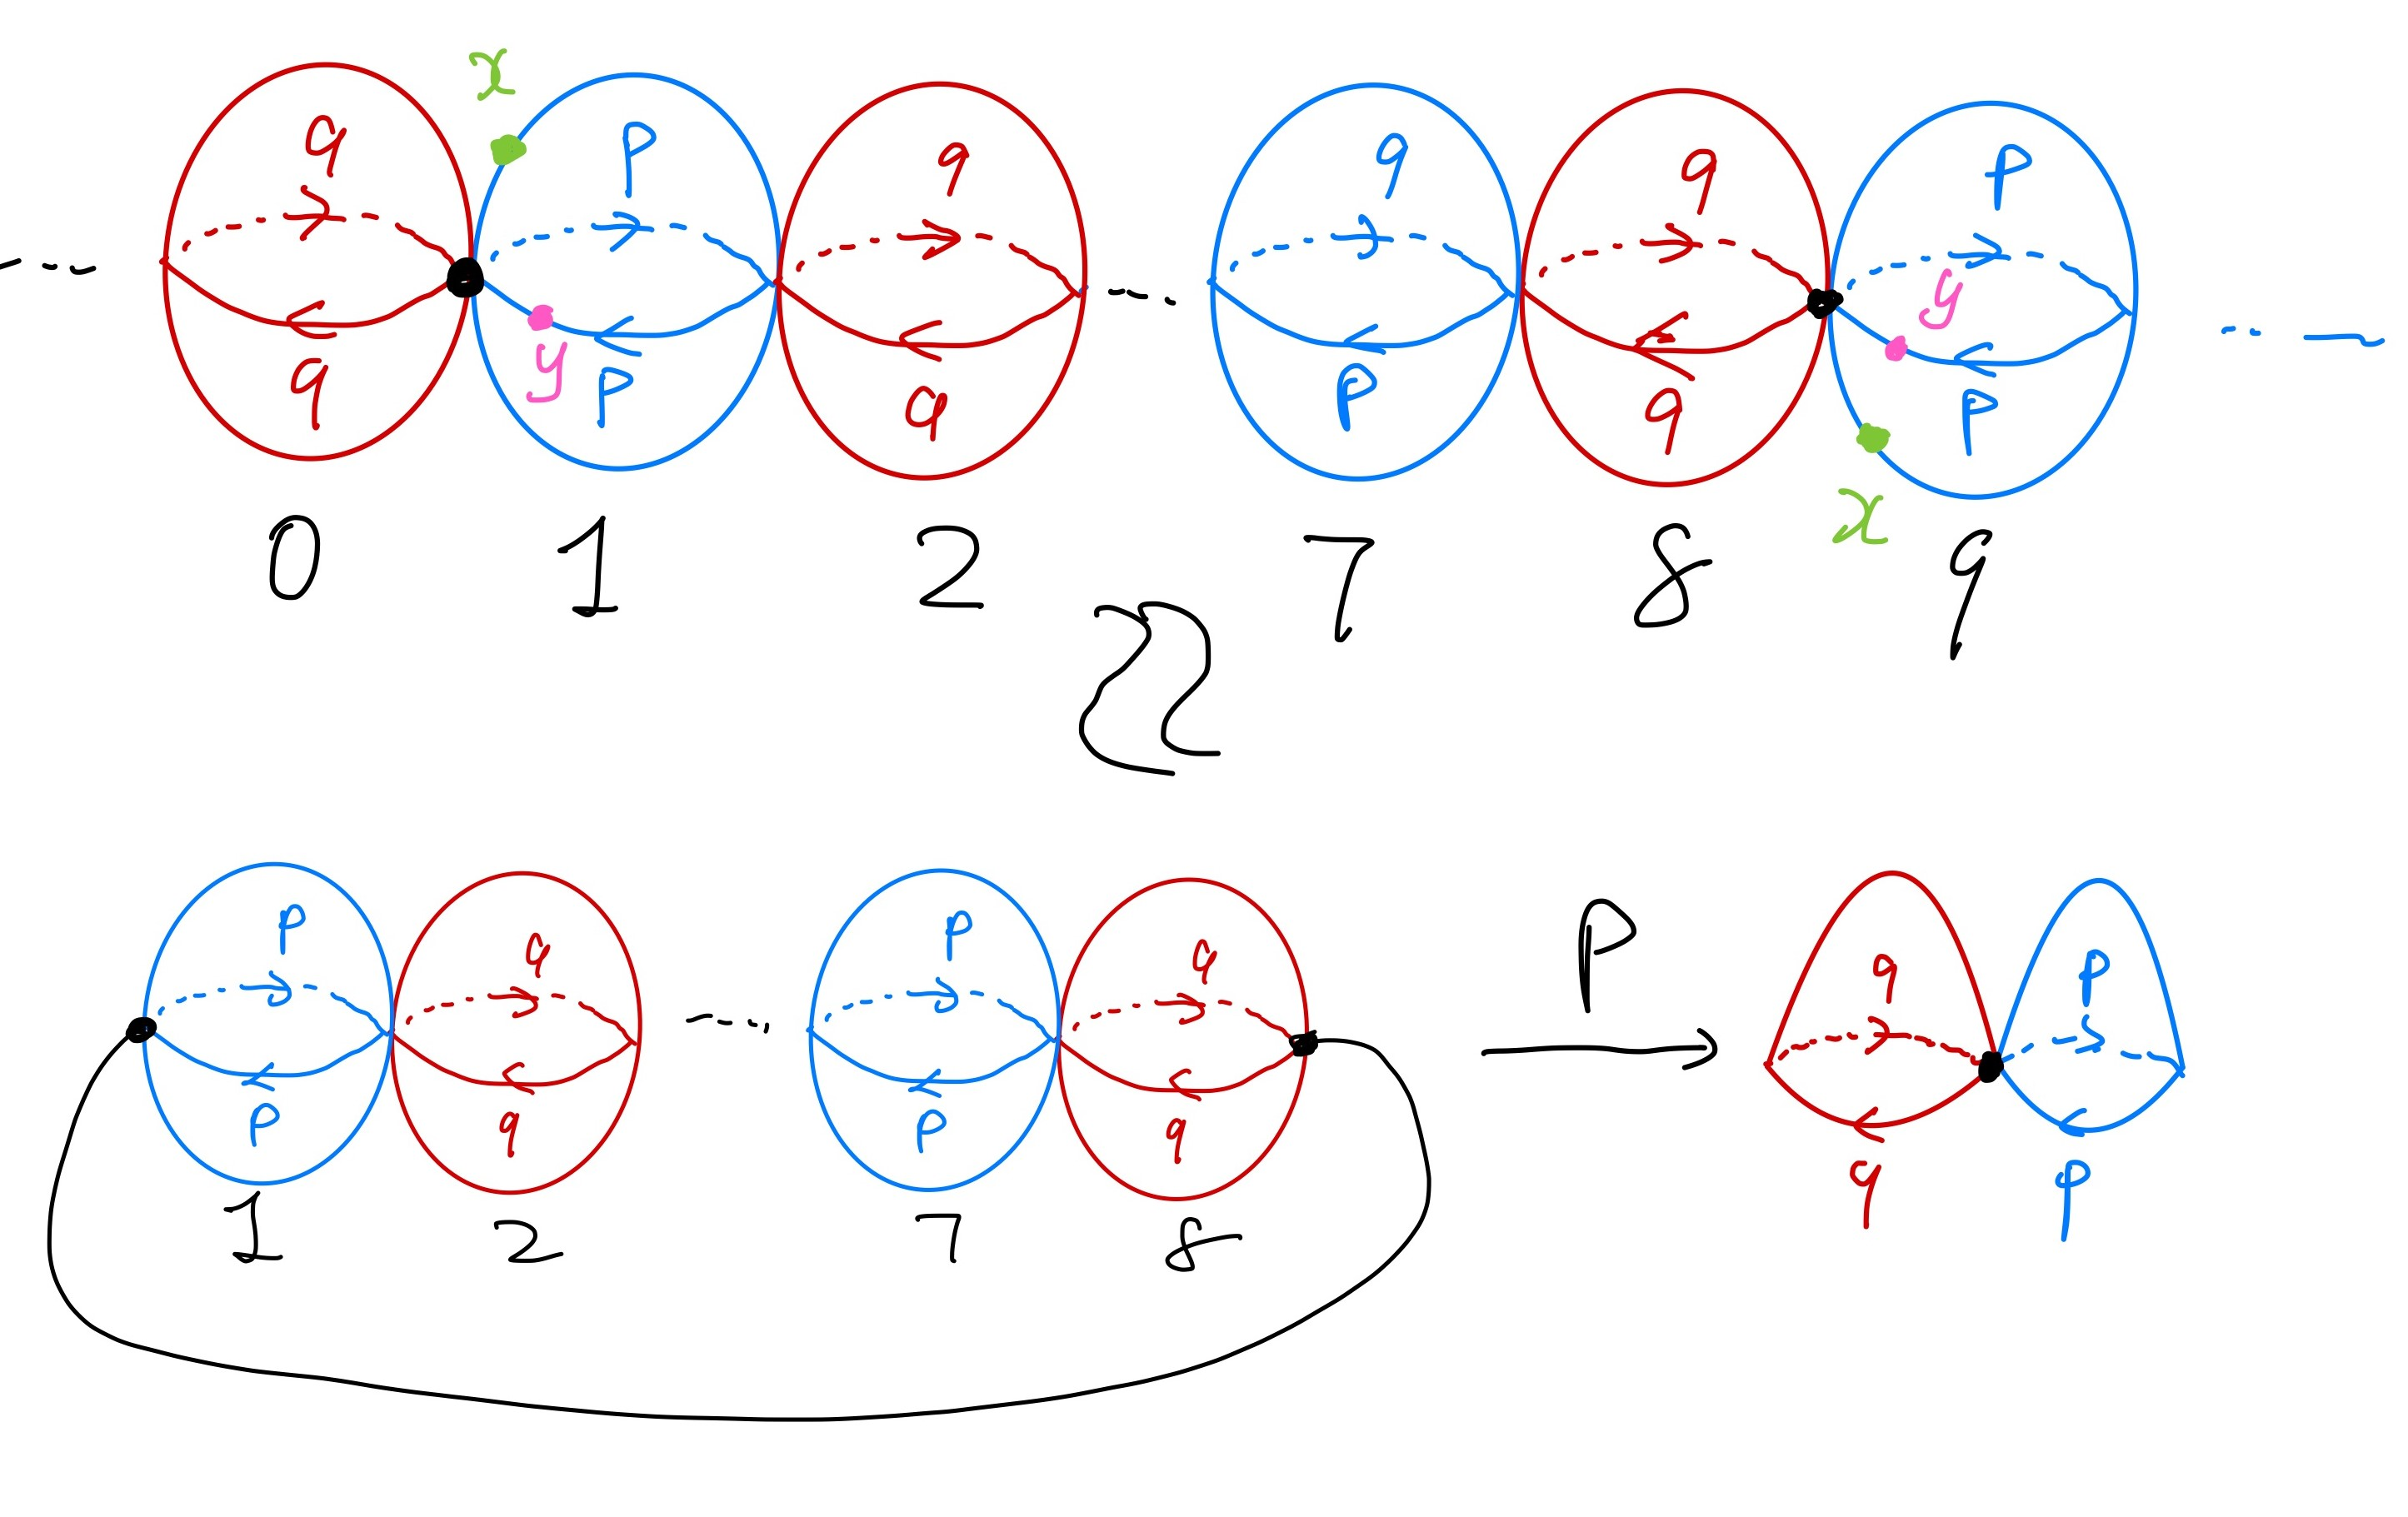
\includegraphics[scale=0.1]{Pictures/HW9-3-1.jpg}\]
From the picture we can see that \(\ti{B}/\la (pq)^4\ra\) is homotopic equivalent to eight \(S^2\) wedged together with a line connecting the starting and ending point. This is homotopic equivalent to 
\((\vee_8 S^2)\vee S^1\). So the homology groups are 
\[H_i(\ti{B}/\la (pq)^4\ra)=\begin{cases}
	\mathbb{Z}^8,&\iif i=2,\\
	\mathbb{Z},&\iif i=0,1,\\ 
	0,&\otherwise.
\end{cases}\]
\item Consider the group \(G\) acts on the following Cayley graph of size 4:
% https://q.uiver.app/#q=WzAsNCxbMCwwLCJzXzEiXSxbMSwwLCJzXzIiXSxbMiwwLCJzXzMiXSxbMywwLCJzXzQiXSxbMCwxLCJwIiwyLHsiY3VydmUiOjIsImNvbG91ciI6WzIzMCw4Niw2MF19LFsyMzAsODYsNjAsMV1dLFsxLDAsInAiLDIseyJjdXJ2ZSI6MiwiY29sb3VyIjpbMjMwLDg2LDYwXX0sWzIzMCw4Niw2MCwxXV0sWzEsMiwicSIsMix7ImN1cnZlIjoyLCJjb2xvdXIiOlswLDYwLDYwXX0sWzAsNjAsNjAsMV1dLFsyLDEsInEiLDIseyJjdXJ2ZSI6MiwiY29sb3VyIjpbMCw2MCw2MF19LFswLDYwLDYwLDFdXSxbMiwzLCJwIiwyLHsiY3VydmUiOjIsImNvbG91ciI6WzIzMCw4Niw2MF19LFsyMzAsODYsNjAsMV1dLFszLDIsInAiLDIseyJjdXJ2ZSI6MiwiY29sb3VyIjpbMjMwLDg2LDYwXX0sWzIzMCw4Niw2MCwxXV0sWzAsMCwicSIsMCx7ImFuZ2xlIjotOTAsImNvbG91ciI6WzAsNjAsNjBdfSxbMCw2MCw2MCwxXV0sWzMsMywicSIsMCx7ImFuZ2xlIjo5MCwiY29sb3VyIjpbMCw2MCw2MF19LFswLDYwLDYwLDFdXV0=
\[\begin{tikzcd}
	{s_1} & {s_2} & {s_3} & {s_4}
	\arrow["q", color={rgb,255:red,214;green,92;blue,92}, from=1-1, to=1-1, loop, in=145, out=215, distance=10mm]
	\arrow["p"', color={rgb,255:red,65;green,95;blue,241}, curve={height=12pt}, from=1-1, to=1-2]
	\arrow["p"', color={rgb,255:red,65;green,95;blue,241}, curve={height=12pt}, from=1-2, to=1-1]
	\arrow["q"', color={rgb,255:red,214;green,92;blue,92}, curve={height=12pt}, from=1-2, to=1-3]
	\arrow["q"', color={rgb,255:red,214;green,92;blue,92}, curve={height=12pt}, from=1-3, to=1-2]
	\arrow["p"', color={rgb,255:red,65;green,95;blue,241}, curve={height=12pt}, from=1-3, to=1-4]
	\arrow["p"', color={rgb,255:red,65;green,95;blue,241}, curve={height=12pt}, from=1-4, to=1-3]
	\arrow["q", color={rgb,255:red,214;green,92;blue,92}, from=1-4, to=1-4, loop, in=325, out=35, distance=10mm]
\end{tikzcd}\]
This corresponds to the following path-connected covering space. 
\[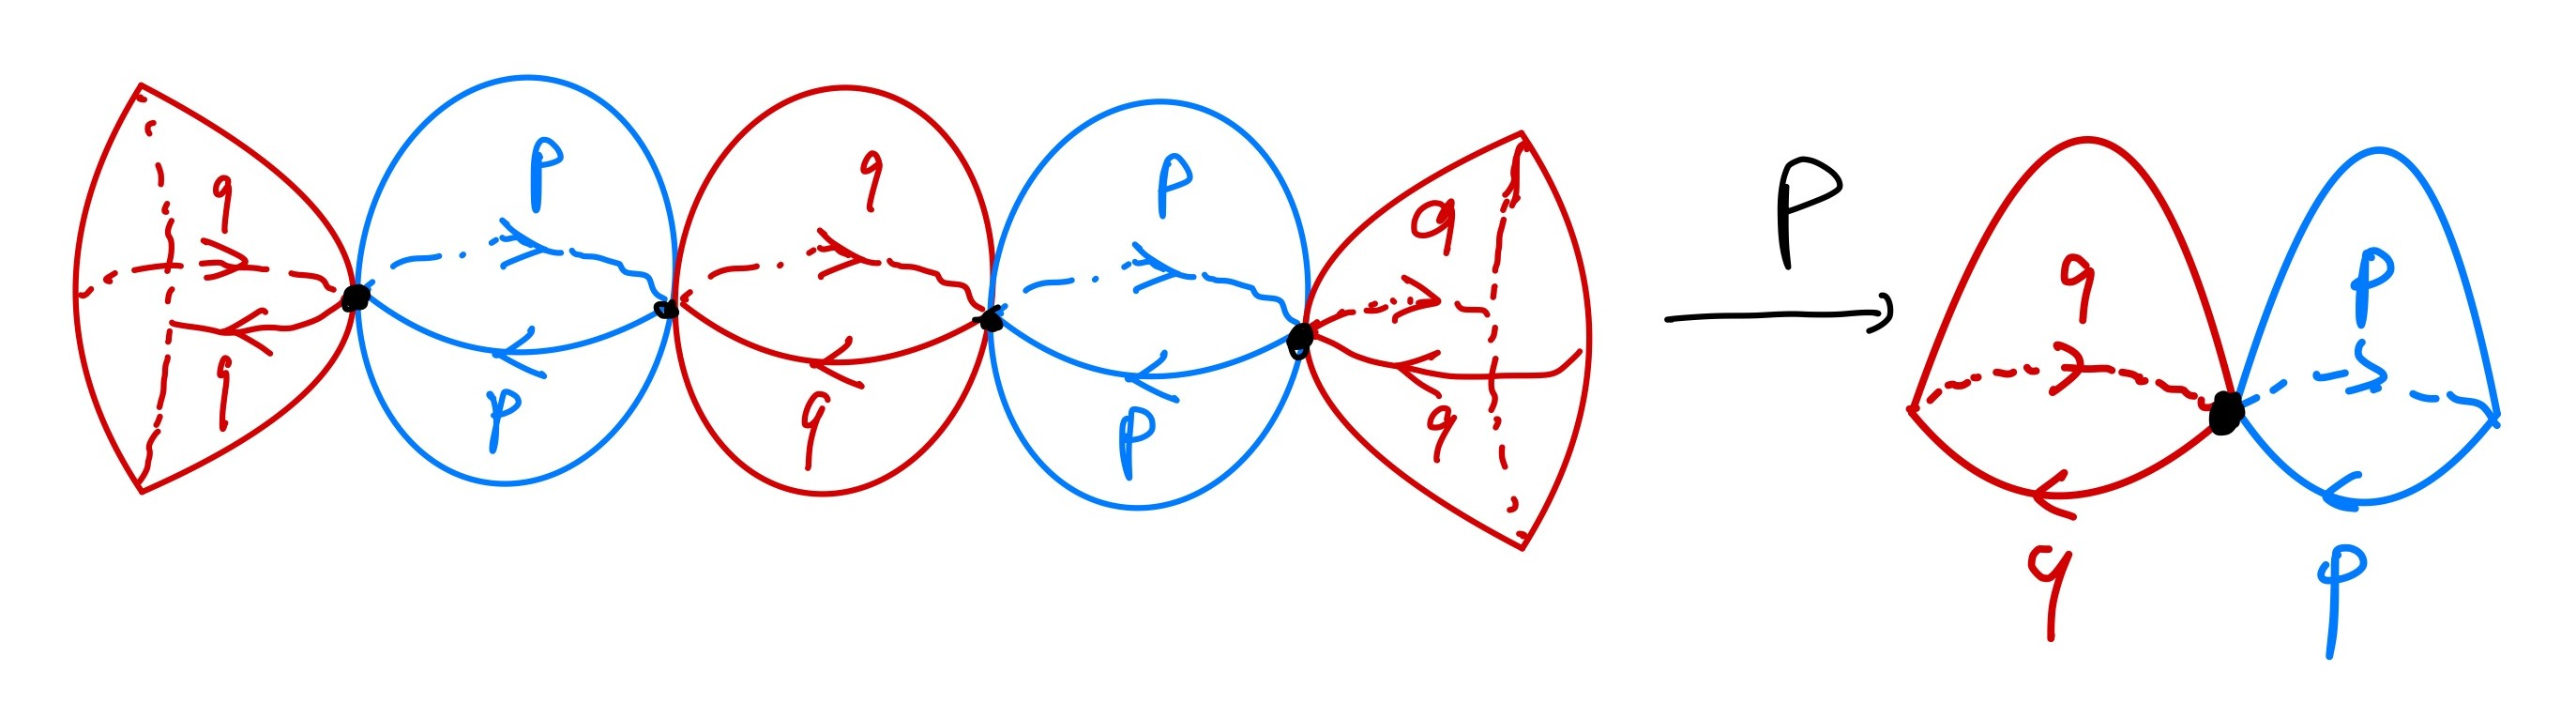
\includegraphics[scale=0.1]{Pictures/HW9-3-2.jpg}\]
Note that \(\Stab(s_1)=\la q, p^2\ra\) and \(\Stab(s_2)=\la p^2,q^2\ra\). They have different stabilizers, so this is not a regular covering space.
\end{enumerate}
\end{solution}

\noindent\rule{7in}{2.8pt}
%%%%%%%%%%%%%%%%%%%%%%%%%%%%%%%%%%%%%%%%%%%%%%%%%%%%%%%%%%%%%%%%%%%%%%%%%%%%%%%%%%%%%%%%%%%%%%%%%%%%%%%%%%%%%%%%%%%%%%%%%%%%%%%%%%%%%%%%
%Probelm 4
%%%%%%%%%%%%%%%%%%%%%%%%%%%%%%%%%%%%%%%%%%%%%%%%%%%%%%%%%%%%%%%%%%%%%%%%%%%%%%%%%%%%%%%%%%%%%%%%%%%%%%%%%%%%%%%%%%%%%%%%%%%%%%%%%%%%%%%5
\begin{problem}{4}
Prove that the genus 2 torus does not admit a path-connected, regular covering space whose automorphism group is \((\mathbb{Z}/3)^5\).
\end{problem}
\begin{solution}
Let \(B\) be the genus \(2\) torus and \(B\) has a CW structure as follows 
\[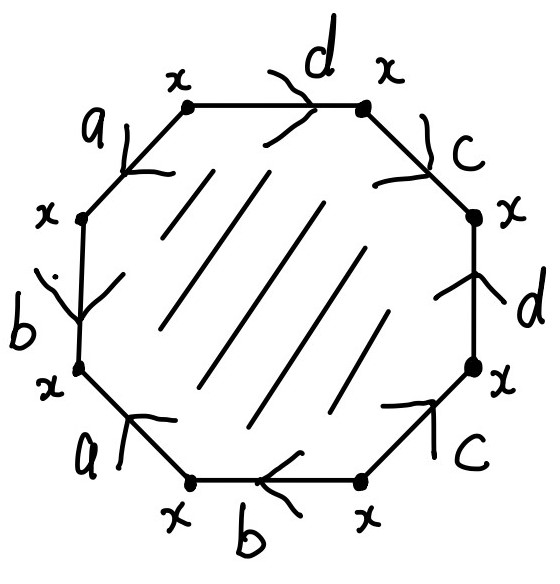
\includegraphics[scale=0.5]{Pictures/HW9-4-1.jpg}\]
The fundamental group \(G\) can be calculated 
\[G=\pi_1(B)=\la a,b,c,d\mid bab^{-1}a^{-1}dcd^{-1}c^{-1}=1\ra\]
Assume we have a path-connected, regular covering space \(p:E\rightarrow B\). It is regular so the automorphism group \((\mathbb{Z}/3)^5=\Aut_B(E)\cong G/H\) for some normal subgroup \(H\). We have a surjective group homomorphism 
\(f:G\twoheadrightarrow (\mathbb{Z}/3)^5\). Note that \((\mathbb{Z}/3)^5\) is an abelian group,  so the map \(f\) must factor through the abelianization \(\pi_1(B)_{ab}=\la a,b,c,d\ra=\mathbb{Z}^4\). Moreover, every element in \((\mathbb{Z}/3)^5\) has order 3 except the identity element, so 
the map must factor through \((\mathbb{Z}/3)^4\), we have an commutative diagram 
% https://q.uiver.app/#q=WzAsMyxbMCwwLCJHIl0sWzEsMCwiKFxcbWF0aGJie1p9LzMpXjUiXSxbMCwxLCIoXFxtYXRoYmJ7Wn0vMyleNCJdLFswLDIsIiIsMCx7InN0eWxlIjp7ImhlYWQiOnsibmFtZSI6ImVwaSJ9fX1dLFsyLDEsIlxcdGlsZGV7Zn0iLDIseyJzdHlsZSI6eyJoZWFkIjp7Im5hbWUiOiJlcGkifX19XSxbMCwxLCJmIiwwLHsic3R5bGUiOnsiaGVhZCI6eyJuYW1lIjoiZXBpIn19fV1d
\[\begin{tikzcd}
	G & {(\mathbb{Z}/3)^5} \\
	{(\mathbb{Z}/3)^4}
	\arrow["f", two heads, from=1-1, to=1-2]
	\arrow[two heads, from=1-1, to=2-1]
	\arrow["{\tilde{f}}"', two heads, from=2-1, to=1-2]
\end{tikzcd}\]
This means we have a surjective map \((\mathbb{Z}/3)^4\rightarrow (\mathbb{Z}/3)^5\), by the structure theorem of abelian groups, this is impossible, so we do not have such a covering.
\end{solution}

\noindent\rule{7in}{2.8pt}
%%%%%%%%%%%%%%%%%%%%%%%%%%%%%%%%%%%%%%%%%%%%%%%%%%%%%%%%%%%%%%%%%%%%%%%%%%%%%%%%%%%%%%%%%%%%%%%%%%%%%%%%%%%%%%%%%%%%%%%%%%%%%%%%%%%%%%%%
%Probelm 5
%%%%%%%%%%%%%%%%%%%%%%%%%%%%%%%%%%%%%%%%%%%%%%%%%%%%%%%%%%%%%%%%%%%%%%%%%%%%%%%%%%%%%%%%%%%%%%%%%%%%%%%%%%%%%%%%%%%%%%%%%%%%%%%%%%%%%%%%
\begin{problem}{5}
Recall that one has an isomorphism \(\pi_1(S^1\times S^1)\cong \mathbb{Z}\oplus \mathbb{Z}\) in which the generators \((1,0)\) and \((0,1)\) correspond to the usual fundamental loops in the torus. Describe (preferably by drawing a picture) the 
covering space \(p:E\rightarrow S^1\times S^1\) for which \(p_*(\pi_1(E,e))=\la (2,4)\ra\). In your picture of \(E\), indicate a generator for \(\pi_1(E)\). Identify the group \(\Aut(E)\), and give a geometric description of some generators for this 
group in terms of your picture.
\end{problem}
\begin{solution}
Let \(T=S^1\times S^1\) be the torus and \(G=\pi_1(T)=\mathbb{Z}\oplus \mathbb{Z}\) be its fundamental group with generators \((1,0)\) and \((0,1)\). Conisder the universal covering space \(\ti{p}:\mathbb{R}^2\rightarrow T\). Write \(b\in T\) as the base point in \(T\). Establish an coordinate system in \(\mathbb{R}^2\), the point 
\((0,0)\) is the base point in \(\mathbb{R}^2\) and the integer points are the fiber \(\ti{p}^{-1}(b)\) over \(b\in T\). By the classification theorem for covering spaces over \(T\), the subgroup \(\la (2,4)\ra\) corresponds to the covering space \(E=\mathbb{R}^2/\la (2,4)\ra\). This is an abelian group, so the orbit space under this group action 
is the same as the quotient space 
\[\mathbb{R}^2/\sim\cong S^1\times \mathbb{R}\]
where \((x,y)\sim (x+2,y+4)\) for all \((x,y)\in \mathbb{R}^2\). As shown in the following picture, this gives us an infinite cylinder 
\[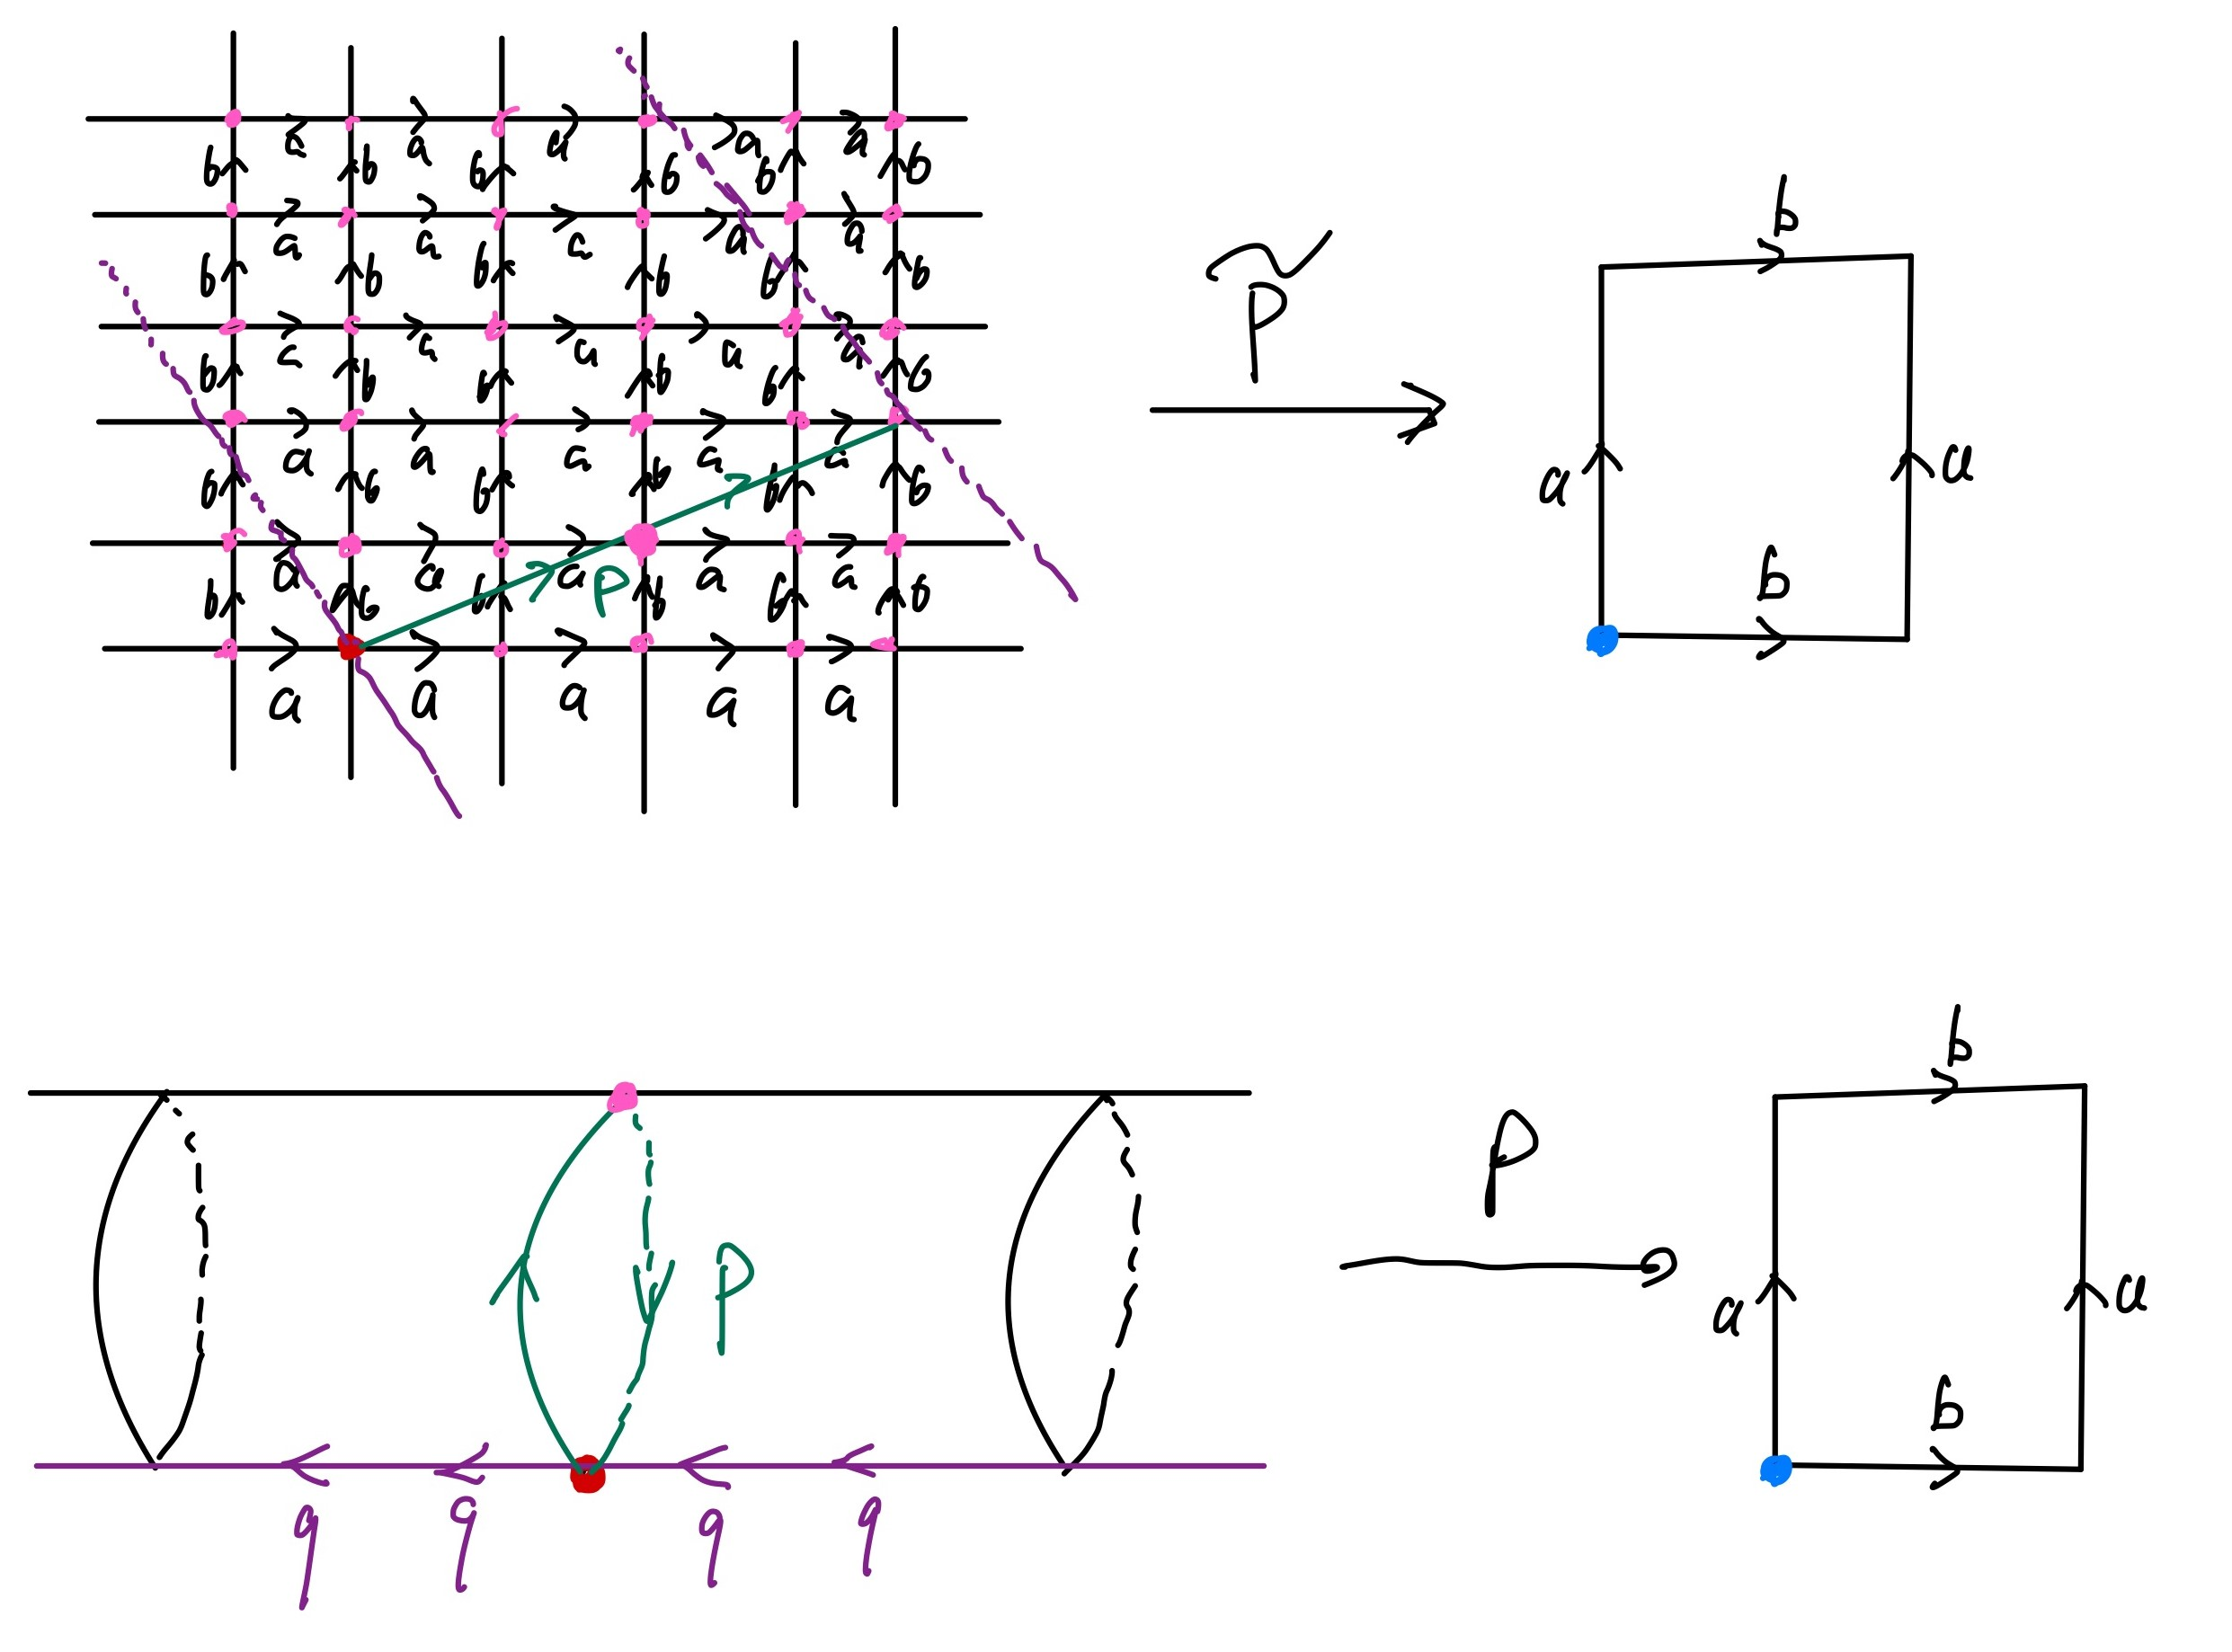
\includegraphics[scale=0.15]{Pictures/HW9-5-1.jpg}\]
The generator for \(\pi_1(E)\) can be viewed as a straight line in the \(\mathbb{R}^2\) grid from the point \((0,0)\) to \((2,4)\) (they get identified in the quotient space \(E\)). Or the green circles in the infinite cylinders. Moreover, since \(G\) is abelian, every subgroup is normal, so the covering \(p:E\rightarrow T\) is normal. We have 
\(\Aut_T(E)\cong G/\la (2,4)\ra\), which is 
\[\Aut_T(E)=\la (1,0),(0,1)\ra/\la (2,4)\ra=\la (1,2),(0,1)\ra/\la (2,4)\ra\cong \mathbb{Z}/2 \mathbb{Z}\oplus \mathbb{Z}.\]
Suppose \(\Aut_T(E)\) has two generators \(p\) and \(q\) with \(p^2=1\) and \(\la q\ra=\mathbb{Z}\). For the \(\mathbb{R}^2/\sim\) model, \(p\) corresponds to the translation of \(\mathbb{R}^2\) in the direction from \((0,0)\) to \((1,2)\) (green line), \(q\) corresponds to the translation in the direction perpendicular to the green line (purple line). For the 
infinite cylinder model \(S^1\times \mathbb{R}\), \(p\) corresponds to the rotation by \(180\) degrees (red point to pink point), and \(q\) corresponds to the translation along with the \(\mathbb{R}\) direction (purple).
\end{solution}

\noindent\rule{7in}{2.8pt}
%%%%%%%%%%%%%%%%%%%%%%%%%%%%%%%%%%%%%%%%%%%%%%%%%%%%%%%%%%%%%%%%%%%%%%%%%%%%%%%%%%%%%%%%%%%%%%%%%%%%%%%%%%%%%%%%%%%%%%%%%%%%%%%%%%%%%%%%
%Probelm 6
%%%%%%%%%%%%%%%%%%%%%%%%%%%%%%%%%%%%%%%%%%%%%%%%%%%%%%%%%%%%%%%%%%%%%%%%%%%%%%%%%%%%%%%%%%%%%%%%%%%%%%%%%%%%%%%%%%%%%%%%%%%%%%%%%%%%%%%%
\begin{problem}{6}
Let \(T\) be the torus, and \(p:\mathbb{R}^2\rightarrow T\) the map \(p(x,y)=(e^{2\pi i x},e^{2\pi i y})\).
\begin{enumerate}[(a)]
\item Let \(\sigma:T\rightarrow T\) be an automorphism that fixes \(p(0,0)\in T\). Using covering space theory (or otherwise), prove that there is an automorphism \(\phi:\mathbb{R}^2\rightarrow \mathbb{R}^2\) such that \(\phi(0,0)=(0,0)\) and the diagram 
% https://q.uiver.app/#q=WzAsNCxbMCwwLCJcXG1hdGhiYntSfV4yIl0sWzEsMCwiXFxtYXRoYmJ7Un1eMiJdLFswLDEsIlQiXSxbMSwxLCJUIl0sWzIsMywiXFxzaWdtYSJdLFswLDJdLFsxLDNdLFswLDEsIlxccGhpIl1d
\[\begin{tikzcd}
	{\mathbb{R}^2} & {\mathbb{R}^2} \\
	T & T
	\arrow["\phi", from=1-1, to=1-2]
	\arrow[from=1-1, to=2-1]
	\arrow[from=1-2, to=2-2]
	\arrow["\sigma", from=2-1, to=2-2]
\end{tikzcd}\]
commutes. If \(\sigma^n=id\), explain why \(\phi^n=id\).
\item Let \(X\) be the quotient space \((T\times I)/\sim \), where the quotient relation has \((t,1)\sim (\sigma(t),0)\). Describe as best you can, the universal covering space of \(X\). 
\item Prove that \(\pi_1(X)\) contains \(\mathbb{Z}^2\) as a subgroup. If \(\phi(x)=Ax\) for some non-identity matrix \(A\) in \(GL_2(\mathbb{Z})\), prove that \(\pi_1(X)\) is non-abelian. 
\item What is \(\pi_3(X)\)?
\end{enumerate}
\end{problem}
\begin{solution}
\begin{enumerate}[(a)]
\item Let \(p:\mathbb{R}^2\rightarrow T\) be the universal covering space of the torus \(T\). Consider the following diagram of pointed spaces: 
% https://q.uiver.app/#q=WzAsNCxbMCwxLCJcXG1hdGhiYntSfV4yIl0sWzEsMSwiVCJdLFsyLDEsIlQiXSxbMiwwLCJcXG1hdGhiYntSfV4yIl0sWzAsMSwicCIsMl0sWzEsMiwiXFxzaWdtYSIsMl0sWzMsMiwicCJdLFswLDMsIlxccGhpIiwwLHsic3R5bGUiOnsiYm9keSI6eyJuYW1lIjoiZGFzaGVkIn19fV1d
\[\begin{tikzcd}
	&& {\mathbb{R}^2} \\
	{\mathbb{R}^2} & T & T
	\arrow["p", from=1-3, to=2-3]
	\arrow["\exists !\phi", dashed, from=2-1, to=1-3]
	\arrow["p"', from=2-1, to=2-2]
	\arrow["\sigma"', from=2-2, to=2-3]
\end{tikzcd}\]
Write \(b=p(0,0)\in T\) as the base point in the torus. It is easy to check that 
\[\sigma(p(0,0))=\sigma(b)=b=p(0,0).\]
By the map lifting lemma, there exists a unique \(\phi:\mathbb{R}^2\rightarrow \mathbb{R}^2\) such that \(p\phi=\sigma p\) and \(\phi(0,0)=(0,0)\) (the base point is mapped to the base point). Now assume \(\sigma^n=id\), consider the following diagram 
% https://q.uiver.app/#q=WzAsNCxbMCwxLCJcXG1hdGhiYntSfV4yIl0sWzEsMSwiVCJdLFsyLDEsIlQiXSxbMiwwLCJcXG1hdGhiYntSfV4yIl0sWzAsMSwicCIsMl0sWzEsMiwiXFxzaWdtYV5uPWlkIiwyXSxbMywyLCJwIl0sWzAsMywiXFxwaGkiLDAseyJzdHlsZSI6eyJib2R5Ijp7Im5hbWUiOiJkYXNoZWQifX19XV0=
\[\begin{tikzcd}
	&& {\mathbb{R}^2} \\
	{\mathbb{R}^2} & T & T
	\arrow["p", from=1-3, to=2-3]
	\arrow["\phi", dashed, from=2-1, to=1-3]
	\arrow["p"', from=2-1, to=2-2]
	\arrow["{\sigma^n=id}"', from=2-2, to=2-3]
\end{tikzcd}\]
By the map lifting lemma, we know that \(id:\mathbb{R}^2\rightarrow \mathbb{R}^2\) is the unique map making the diagram commutes. On the other hand, consider the following diagram 
% https://q.uiver.app/#q=WzAsNCxbMCwxLCJUIl0sWzEsMSwiVCJdLFswLDAsIlxcbWF0aGJie1J9XjIiXSxbMSwwLCJcXG1hdGhiYntSfV4yIl0sWzAsMSwiXFxzaWdtYV5uIiwyXSxbMiwwLCJwIiwyXSxbMywxLCJwIl0sWzIsMywiXFxwaGlebiJdXQ==
\[\begin{tikzcd}
	{\mathbb{R}^2} & {\mathbb{R}^2} \\
	T & T
	\arrow["{\phi^n}", from=1-1, to=1-2]
	\arrow["p"', from=1-1, to=2-1]
	\arrow["p", from=1-2, to=2-2]
	\arrow["{\sigma^n}"', from=2-1, to=2-2]
\end{tikzcd}\]
It commutes because 
\[\sigma^np=\sigma^{n-1}(\sigma p)=\sigma^{n-1}p\phi=\cdots=p\phi^n.\]
By the uniqueness of the lifted map, we know that \(\phi^n=id\).
\item The universal space is given by \(p_2:\mathbb{R}^3\rightarrow X\). Write \(\mathbb{R}^3=\mathbb{R}^2\times \mathbb{R}\). For \(\mathbb{R}^2\times \left\{ 0 \right\}\subseteq \mathbb{R}^3\), \(p_2\) can be described as 
\[p_2=p\times id:\mathbb{R}^2\times \left\{ 0 \right\}\rightarrow T\times \left\{ 0 \right\}\]
where \(p:\mathbb{R}^2\rightarrow T\) is the universal covering space of \(T\). For \(\mathbb{R}^2\times \left\{ 1 \right\}\subseteq \mathbb{R}^3\), \(p_2\) can be described as 
\[p_2=p\circ \phi:\mathbb{R}^2\times \left\{ 1 \right\}\rightarrow \mathbb{R}^2\times \left\{ 1 \right\}\rightarrow T\times \left\{ 0 \right\}\]
where \(\phi\) is the lifting from part (a). This is well-defind because we know from (a) that \(p\phi =\sigma p\), so \(p_2\) in this case is the same as 
\[\sigma p=\mathbb{R}^2\times \left\{ 1 \right\}\rightarrow T\times \left\{ 1 \right\}\rightarrow T\times \left\{ 0 \right\}.\]
For any \(0<z<1\), we define \(p_2(x,y)=p(x,y)\) just as the universal covering space \(p:\mathbb{R}^2\rightarrow T\).
For \(0\leq z\leq 1\), we define 
\begin{align*}
	p_2:\mathbb{R}^2\times [0,1]&\rightarrow T\times I/\sim,\\ 
	    ((x,y),z)&\mapsto (p_2(x,y),e^{2\pi iz}).
\end{align*}
Let \(n\in \mathbb{Z}\). Similarly as above, for any \(\mathbb{R}^2\times \left\{ n \right\}\subseteq \mathbb{R}\), we can define 
\[p_2=p\circ \phi^n:\mathbb{R}^2\times \left\{ n \right\}\rightarrow T\times \left\{ 0 \right\}.\]
This is well-defined from our previous discussion and part (a). Now we obtained the whole covering space 
\begin{align*}
	p_2:\mathbb{R}^2\times \mathbb{R}&\rightarrow T\times I/\sim,\\ 
	    ((x,y),z)&\mapsto (p_2(x,y),e^{2\pi iz}).
\end{align*}
Here when \(n-1\leq z<n\), we have \(p_2=p\circ \phi^{n-1}:\mathbb{R}^2\times \left\{ z \right\}\rightarrow T\times \left\{ 0 \right\}\).
\item Note that by the classification theorem for covering space, \(\Aut_X(\mathbb{R}^3)\cong \pi_1(X)/p_{2*}(\pi_1(\mathbb{R}^3))=\pi_1(X)\). And consider the translation of \(\mathbb{R}^3\) by 1 in the \(x\) direction, this defines 
an automorphism of the covering space \(p_2:\mathbb{R}^3\rightarrow X\), and it generates a subgroup isomorphic to \(\mathbb{Z}\) in \(\Aut_X(\mathbb{R}^3)\). Same for the translation in the \(y\) direction by 1. We can see that \(\pi_1(X)\) contains 
\(\mathbb{Z}^2\) as a subgroup. 

Now assume \(A=\phi:\mathbb{R}^2\rightarrow \mathbb{R}^2\) is in \(GL_2(\mathbb{Z})\) and is not the identity matrix. \(A\) defines an automorphism of covering space by sending \((x,y,z)\) to \((A(x,y),z)\). For \(m,n\in \mathbb{Z}\), note that 
\((A(x+m,y+n),z)\neq (A(x,y)+(m,n),z)\) in general, so \(\pi_1(X)\) is not an abelian group. 
\item The covering space \(\mathbb{R}^3\xrightarrow{p_2}X\) is a fiber bundle and we have a long exact sequence in homotopy groups. The fiber is discrete so for \(i\geq 2\), we have 
\[\pi_i(\mathbb{R}^3)\cong \pi_i(X).\]
When \(i=3\), we have \(\pi_3(X)=0\) is trivial since \(\mathbb{R}^3\) is contractible.
\end{enumerate}
\end{solution}





\end{document}